% This document holds the main content of the talk. It is included in
% the two global documumetns `Presentation.tex` and `Handout.tex` that
% are used to create the actual presentation as well as a two on one
% collated handout of the slides.
%
% All real content has to go to _this_ file!
%
% Last change: <Wed, 2022/02/09 16:12:37 arwagner l00lnxwagner.desy.de>
%
\mode<handout>{%
    \usepackage{pgf}
    \usepackage{pgfpages}
    \pgfpagesuselayout{2 on 1}[a4paper,border shrink=5mm]
}
\mode<presentation>{%
    \usetheme{DESY}
}

% Setup for Beamer
\usepackage{hyperxmp}
% \usepackage[pdfa]{hyperref}
\usepackage{luatextra}
\usepackage{wasysym}
\usepackage{eurosym}
\usepackage{bookmark}
\usepackage{graphicx}
\usepackage{fontspec}

% Force beamer to use Arial. Without this it will fall back to
% Libertine in all ``normal'' text areas. It seems they are not easily
% accessible from the templates.
\usefonttheme{professionalfonts} % using non standard fonts for beamer
\setmainfont[Mapping=tex-text]{Arial}
\setsansfont[Mapping=tex-text]{Arial}

%% Force Arial for math as well like strict CD.
%% However, usually TeX defaults just look way better
% \usepackage{unicode-math}
% \setmathfont{Arial} % for math symbols, can be any other OpenType math font
% \setmathfont[range=\mathup]  {Arial}
% \setmathfont[range=\mathbfup]{Arial Bold}
% \setmathfont[range=\mathbfit]{Arial Bold Italic}
% \setmathfont[range=\mathit]  {Arial Italic}

\usepackage[ngerman,english]{babel}
\usepackage{xspace}
\usepackage{tikz}
\usepackage{fancyvrb}
\tikzset{%
  every overlay node/.style={%
    %draw=black,fill=white,rounded corners,anchor=north west,
    draw=fzjlightblue,fill=fzjgray30,rounded corners,anchor=north west,
  },
}
% Usage:
% \tikzoverlay at (-1cm,-5cm) {content};
% or
% \tikzoverlay[text width=5cm] at (-1cm,-5cm) {content};
\def\tikzoverlay{%
   \tikz[baseline,overlay]\node[every overlay node]
}%

% General new commands an macros
\renewcommand{\emph}[1]{\structure{#1}}

\newcommand{\link}[2]{\href{#1}{~#2}}

\newcommand{\jointwo}{\href{http://join2.de}{\textbf{JOIN$^2$}\xspace}}

\newcommand{\BibTeX}{Bib\TeX}

\newcommand{\Inspec}{{\texttt{Inspec}}\xspace}
\newcommand{\WoS}{{\texttt{Web of Science}}\xspace}
\newcommand{\Scopus}{\texttt{Scopus}\xspace}
\newcommand{\arxiv}{{\texttt{arXiv.org}}\xspace}
\newcommand{\pubmed}{{\texttt{pubmed}}\xspace}

\newcommand{\JabRef}{\link{http://jabref.sf.net}{JabRef}\xspace}
\newcommand{\Companion}[1]{\textit{\link{http://julib.fz-juelich.de/uhtbin/field-search-sort/001/PBYR/213964}{\LaTeX{} Companion}, #1}\xspace}
\newcommand{\pkg}[1]{\emph{\texttt{#1}}\xspace}

\newcommand{\neutralino}{\ensuremath{\tilde{\chi}^0}\xspace}

% general colour definitions
\newcommand{\smallgray}[1]{{\tiny\emph{#1}}}

\newcommand{\idR}{i.~d.~R.\xspace}
\newcommand{\va}{v.~a.\xspace}
\newcommand{\sa}{s.~a.\xspace}
\newcommand{\zB}{z.~B.\xspace}
\newcommand{\zT}{z.~T.\xspace}
\newcommand{\eg}{e.~g.\xspace}

\newcommand{\bs}[1]{\texttt{$\backslash$#1}}
\newcommand{\command}[2]{\texttt{\bs{#1}\{#2\}}}

\newcommand{\invenio}{\href{http://invenio-software.org}{\raisebox{-0.5em}{\includegraphics[height=1.5em]{pictures/Logo_invenio}}}}
\newcommand{\github}{\href{http://github.com}{%
	\raisebox{-1em}{\includegraphics[height=2.0em]{pictures/Octocat}}%
	\raisebox{-0.5em}{\includegraphics[height=1.5em]{pictures/GitHub_Logo}}}}

\newcommand{\newitem}{\raisebox{-0.7ex}{\includegraphics[height=3ex]{img/new_icon}}}
\newcommand{\newicon}{\raisebox{-1.1ex}{\includegraphics[height=4ex]{img/new_icon}}}
\newcommand{\verytiny}[1]{{\fontsize{3}{4}\selectfont{#1}}}

\newcommand{\DESYWord}{%
\raisebox{0.0px}{%
	\usebeamercolor[fg]{title}{\textbf{DESY}}%
	\usebeamercolor[fg]{subtitle}{\textbf{.}}
}\hspace*{0.2em}
}

\newcommand{\MailTo}[1]{\href{mailto:#1}{#1}}
\newcommand{\DOIlink}[1]{\href{https://doi.org/#1}{\emph{#1}}}
\newcommand{\ORCiD}[1]{
\includegraphics[height=1.5ex]{img/orcid}\,\href{https://www.orcid.org/#1}{#1}}

%%--%% % http://tex.stackexchange.com/questions/16447/beamer-top-aligning-columns-within-a-top-aligned-fram
\makeatletter
\newenvironment{topitemize}{%
   \setlength{\topsep}{0pt}
   \setlength{\partopsep}{0pt}
   \renewcommand*{\@listi}{\leftmargin\leftmargini \parsep\z@ \topsep\z@ \itemsep\z@}
   \let\@listI\@listi
   \itemize
}{\enditemize}
\makeatother

%------------------- Begin of edit -----------------------------------
%
% Adopt the follwing values according to your needs.
%
% Note: improving metadata also improves visibility. Time spent here
% might pay of later. Search engines love keywords, abstracts and
% sensible titles.
%
%     Make sure to submit your talk to the publications database
%         to get a DOI, to make it citable and OpenAccess!
%
\newcommand{\TITLE}{Machine Learning in Quantum Mechanics}     % Title of talk       
\newcommand{\SUBTITLE}{Normalizing Flows for Computing Molecular Vibrational Wave Functions}                 % Subtitle
\newcommand{\AUTHOR}{Nicolas Mendoza}        % your name
\newcommand{\EMAIL}{snmendozav@gmail.com} % your email
\newcommand{\ORCID}{0000--0001--5561--1392}   % your ORCiD
\newcommand{\PHONE}{+49--152--2768--2024}      % your phone number
\newcommand{\GROUP}{CMI}          % your group
\newcommand{\URL}{http://library.desy.de}     % your groups page
\newcommand{\DOI}{10.3204/PUBDB-20YY-nnnn}    % submit and release in pubdb to get a DOI
\newcommand{\INSTITUTE}{DESY} % not used in CD 2018
\newcommand{\CITY}{Hamburg}                      % City of talk
\newcommand{\DATE}{07.09.2022}                % Date of Talk

% To improve visibility - add metadata to the PDF
% - Add sensible keywords describing the topic
% - Add the abstract (one line, no breaks it is just for indexing)
% - Adopt the licence of your work

\hypersetup{%
	pdfkeywords        = {keyword} {keyword} {keyword},
	pdfsubject         = {Abstract},
	pdfcopyright       = {CC-BY},
	pdflicenseurl      = {http://creativecommons.org/licenses/by/4.0/},
	%% pdfcopyright       = {CC-BY-NC-SA},
	%% pdflicenseurl      = {http://creativecommons.org/licenses/by-nc-sa/4.0/},
	pdftitle           = {\TITLE}
	pdfcreator         = {\AUTHOR},
	pdfcaptionwriter   = {\AUTHOR},
	pdfcontactaddress  = {Notkestraße 85},
	pdfcontactcity     = {Hamburg},
	pdfcontactpostcode = {22607},
	pdfcontactcountry  = {Germany},
	pdfcontactemail    = {\EMAIL},
	pdfcontacturl      = {\URL},
	pdflang            = {en},
	bookmarksopen      = true,
	bookmarksopenlevel = 3,
	hypertexnames      = false,
	linktocpage        = true,
	plainpages         = false,
	breaklinks
}

%------------------- End of edit -------------------------------------

% Derive internal values from above data

\author{\AUTHOR}
\title{\TITLE}
\subtitle{\SUBTITLE}
\institute{}  % not used by DESY CD 2018
\date{\CITY, \DATE}


\newcommand{\Hhat}{\hat{H}}
\newcommand\equalhat{\mathrel{\stackon[1.5pt]{=}{\stretchto{%
\scalerel*[\widthof{=}]{\wedge}{\rule{1ex}{3ex}}}{0.5ex}}}}
\newcommand{\nmax}{N_{\text{max}}}
\newcommand{\inner}[2]{\bra{#1}\mkern-7.7mu\ket{#2}}
\newcommand{\dd}{\text{d}}
%---------------------------------------------------------------------

\begin{document}

\maketitle

% Add a licencse statement to all pages. Adopt this if any other
% licences is used!

%-% CC-BY-NC-SA 4
%-% \setbeamertemplate{slide counter}[showall][]
%-% \setbeamertemplate{footer element1}{%
%-%     \href{http://creativecommons.org/licenses/by-nc-sa/4.0/}{
\includegraphics[height=3ex]{img/CCBYNCSA}}
%-% }

% CC-BY 4, current suggetion for scientific content
\setbeamertemplate{slide counter}[showall][]
\setbeamertemplate{footer element1}{%
    \href{http://creativecommons.org/licenses/by/4.0/}{
\includegraphics[height=3ex]{img/CCBY}}
}

%----------------------------------------------------------------------
% Add manual table of contents
% Two column example
% -% \begin{frame}
% -% \frametitle{Overview}
% -%   \begin{columns}
% -%       \begin{column}{0.4\textwidth}
% -%           \hspace*{-0.97cm}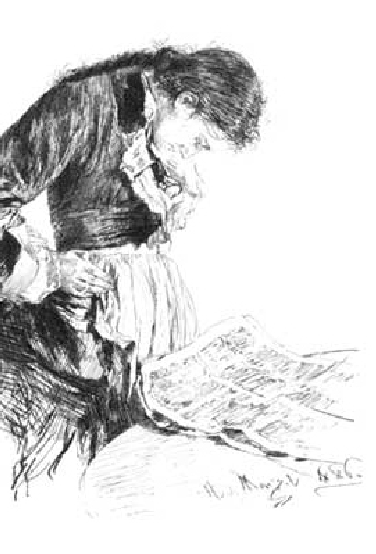
\includegraphics[height=\textheight]{img/menzel}
% -%       \end{column}
% -%       \begin{column}{0.5\textwidth}
% -%           \begin{itemize}[<+->]
% -%               \item {Section}
% -%               \item {Section}
% -%           \end{itemize}
% -%       \end{column}
% -%   \end{columns}
% -% \end{frame}

\begin{frame}
    \frametitle{Overview}
    \begin{itemize}[<+>]
        \item {Introduction}
        \item {Physics}
        \item {Machine Learning}
        \item {Mathematics}
    \end{itemize}
\end{frame}
%----------------------------------------------------------------------
% Missuse parts as chapters according to DESY PR
\part[Part slide]{Introduction}
\makepart%

%----------------------------------------------------------------------
\section{\ldots}

% Add a sample slide with some math, some columns etc.
\begin{frame}[t,label=intro]
\frametitle{The Challenge}

\begin{itemize}[<+->]
    \setlength\itemsep{.8em}
    \item Solving Schrödinger's Equation is \textbf{hard}
    \item Usually turn to numerical approximations
    \item \ldots but numerics have limitations
    \item Amountof data needed depends exponentially on $d$
\end{itemize}

\begin{columns}
    \begin{column}[t]{0.48\textwidth}
        \begin{itemize}[<+->]
            \setlength\itemsep{.8em}
            \item \textit{The Curse of Dimensionality}
            \item How do we improve dependency?
            \item More flexibility to our basis elements 
            \item Machine Learning comes into play
        \end{itemize}
    \end{column}
    \begin{column}[t]{0.48\textwidth}
        \begin{figure}
            \includegraphics[width=\textwidth]{example-image-a}
        \end{figure}
        % Hello there
    \end{column}
\end{columns}

% left aligned columns. Note that columns with smaller width are
% centred automatically

\end{frame}

%----------------------------------------------------------------------
% Missuse parts as chapters according to DESY PR
\part[Part slide]{Physics}
\makepart%

%----------------------------------------------------------------------
% Add a sample slide with some math, some columns etc.
\begin{frame}[t,label=intro]
    \frametitle{Problem Setup}
    \begin{itemize}[<+->]
        \setlength\itemsep{.5em}
        \item Time Independent Schrödiger Equation (\textbf{TISE}) 
        \[ E\ket{\psi} = \Hhat\ket{\psi}\]
        \item We approximate it using the variational principle~~\cite{libretexts_2022}
        \item Fundamentally: We need loss function to optimize
        \item Energy of approximation state $E_\Theta$ is always $\geq$ than groundstate $E_0$
        \begin{proof}
            Assuming normalization of $\ket{\psi_{\Theta}}$ and letting ${\{\ket{k}\}}_{k=1}^\infty$ be eigenstates of $\Hhat$
            \begin{equation}
                E_\Theta = \bra{\psi_{\Theta}}\Hhat\ket{\psi_{\Theta}} = 
                \sum_{m, n = 0}^\infty \bar{\alpha}_m \alpha_n 
                \underbrace{\bra{m}\Hhat\ket{n}}_{E_n\cdot \delta_{m,n}}
                = \sum_{n=0}^\infty |\alpha_n|^2 E_n \geq E_0 \sum_{n=0}^\infty |\alpha_n|^2  = E_0
                \label{eq:larger_than_groundstate_E}
            \end{equation}
        \end{proof}
    \end{itemize}
\end{frame}

\begin{frame}
    \frametitle{Variational Principle}
    \begin{itemize}[<+->]
        \setlength\itemsep{0.9em}
        \item This principle applies to higher order eigenenergies
        \item Idea: Consider orthogonal subspace to $\ket{0}$ and reapply~\eqref{eq:larger_than_groundstate_E}
        \item Can be done for all space (if it is separable)
        \item More rigorous approach in~\cite{libretexts_2022}
        \item $\Rightarrow$ must diagonalize ${[\widetilde{H}]}_{ij}=\bra{\varphi_i}\Hhat\ket{\varphi_j}$
                given arbitrary orthonormal basis ${\{\ket{\varphi_k}\}}_{k=1}^\infty$
        \item Can be an infinite dimensional matrix
        \item $\infty$ is a problem numerically
    \end{itemize}
\end{frame}

\begin{frame}
    \frametitle{Managing $\infty$}
    \begin{itemize}[<+->]
        \setlength\itemsep{0.8em}
        \item Define a truncation parameter $\nmax$
        \item Approximate state as \[\ket{\psi} \approx \sum_{k=0}^{\nmax} c_k \ket{\varphi_k}\]
        \item Becomes finite-dimensional problem
        \item Recall: Curse of dimensionality!
        \item $\nmax$ needed to converge to real results scales \textit{exponentially} with $d$
        \item Approach: define a more flexible `augmented basis' ${\{\ket{\varphi_i^A}\}}_i$ 
        \item Reduce $\nmax$ needed when augmented basis is optimized
    \end{itemize}
\end{frame}


% left aligned columns. Note that columns with smaller width are
% centred automatically
% \begin{columns}
%     \begin{column}[t]{0.48\textwidth}
%     Duis autem vel eum iriure dolor in hendrerit in vulputate velit
%     esse molestie consequat, vel illum dolore eu feugiat nulla
%     facilisis at vero eros et accumsan\ldots
%     \end{column}
%     \begin{column}[t]{0.48\textwidth}
%     Nam liber tempor cum soluta nobis eleifend option congue nihil
%     imperdiet \ldots
%     \end{column}
% \end{columns}


%----------------------------------------------------------------------
% Missuse parts as chapters according to DESY PR
\part[Part slide]{Machine Learning}
\makepart%


\begin{frame}
    \frametitle{Role of ML}
    \begin{itemize}[<+->]
        \setlength\itemsep{1em}
        \item Will start considering coordinate space: $\ket{\psi} \equiv \psi(x)$
        \item Define augmented basis as:
            \begin{equation}
                \varphi_k^A(x) = \varphi_k(g(x)) \cdot \sqrt{\det\left|\frac{\dd g}{\dd x}\right|}
            \end{equation}
        \item $g$ is a \textbf{Normalizing Flow}
        \item This preserves orthonormality
            \begin{proof}
                \[
                    \inner{\varphi_k^A(x)}{\varphi_k^A(x)} = 
                    \int \dd x \varphi_i(g(x))\varphi_j(g(x)) \cdot \det\left|\frac{\dd g}{\dd x}\right|=
                    \int \dd g \left|\frac{\dd x}{\dd g}\right| \varphi_i(g)\varphi_j(g) \cdot \det\left|\frac{\dd g}{\dd x}\right|= \delta_{i, j}
                \]
            \end{proof} 
    \end{itemize}
\end{frame}

\begin{frame}
    \frametitle{Normalizing Flows}
    \begin{itemize}[<+->]
        \setlength\itemsep{1em}
        \item Basic idea: A chain of diffeomorphisms
        \item Invertible and differentiable
        \begin{equation*}
            \boldmath{z} = (f_n\circ f_{n-1} \circ \dots \circ f_1 )(\boldmath{x})
        \end{equation*}
        \item Several different paradigms
        \item Need to find which ones best improve flexibility of basis states
        \item We concentrate on RNVP 
    \end{itemize}
\end{frame}

\begin{frame}
    \frametitle{RNVP}
    \begin{itemize}
        \setlength\itemsep{.6em}
        \item The Real-valued Non-Volume-Preserving Normalizing Flow
        \item Let $\mathcal{P}_k$ be a projection over half of the basis vectors and $\mathcal{Q}_k \equiv \mathbb{1} - \mathcal{P}_k$
        \item layer $g_k(x)$ is given by 
            \begin{equation}
                g_k(x) = \mathcal{P}_k[x] + \mathcal{Q}_k [f_k(x)] \quad \text{with} \quad f_k(x) =  e^{s_k(\mathcal{P}_k[x])} \odot x + t_k(\mathcal{P}_k[x])
                \label{eq:layer_RNVP}
            \end{equation}
        % \item The inverse of $g \equiv g_M\circ g_{M-1}\circ \dots \circ g_1$ is $g^{-1} = g_M^{-1} \circ g_{M-1}^{-1} \circ \dots \circ g_1^{-1}$
    \end{itemize}
    \begin{columns}
        \begin{column}[t]{0.48\textwidth}
            \begin{itemize}
                \item Each $g_k$ is invertible: 
                \[
                    g_k^{-1}(z) = \mathcal{P}_k[z] + \mathcal{Q}_k[f_k^{-1}(z)] 
                \]
                \[ 
                    \text{with} \quad f_k^{-1}(z) =  e^{-s_k(\mathcal{P}_k[z])} \odot (z - t_k(\mathcal{P}_k[z]))
                \]
                \item Can be shown rigorously
                % \item sub Recall that for a projection $\mathcal{P}$, we have $\mathcal{P}^2 = \mathcal{P}$
                % \item sub Using linearity of $\mathcal{Q}$ and noticing it commutes with diagonal matrices
            \end{itemize}
        \end{column}

        \begin{column}[t]{0.48\textwidth}
            \begin{figure}
                \includegraphics[scale=0.3]{example-image-b}
            \end{figure} 
        \end{column}
    \end{columns}

\end{frame}
\begin{frame}
    \frametitle{Convergence}
    How do we know $\displaystyle{\sum_{k=0}^{\nmax}c_k \varphi_k^A}$ converges to the real result as ${\nmax} \to \infty$?
    \begin{itemize}
        \item Let $g$ be the normalizing flow
        \item Analogous to showing $f \circ g \in \mathcal{S}\,\, \forall f \in \mathcal{S}$
        \item $\mathcal{S}$ are rapidly decreasing, infinitely differentiable functions
        \item \[ \equiv f \in C^\infty | \|x^\beta \cdot \frac{\partial^\alpha}{\partial^\alpha}\| < \infty \]
        \item If $g$ is RNVP (with a slight modification), then $f \circ g \in \mathcal{S}$
        \item \textit{Proof left as an exercise to the reader}
    \end{itemize}
\end{frame}
\begin{frame}
    \frametitle{Performance?}
    \begin{columns}
        \begin{column}[t]{0.48\textwidth}
            \begin{itemize}
                \setlength\itemsep{.8em}
                \item We compared results in H2S molecule
                \item Normalizing Flows greatly improved stretching case (Fig.~\ref{fig:enrs_stretch_2D})
                \item RNVP behaves similarly to IResNet
                \item Possibly perform better on higher dimensional data
            \end{itemize}
        \end{column}
        \begin{column}[t]{0.48\textwidth}
            \begin{figure}
                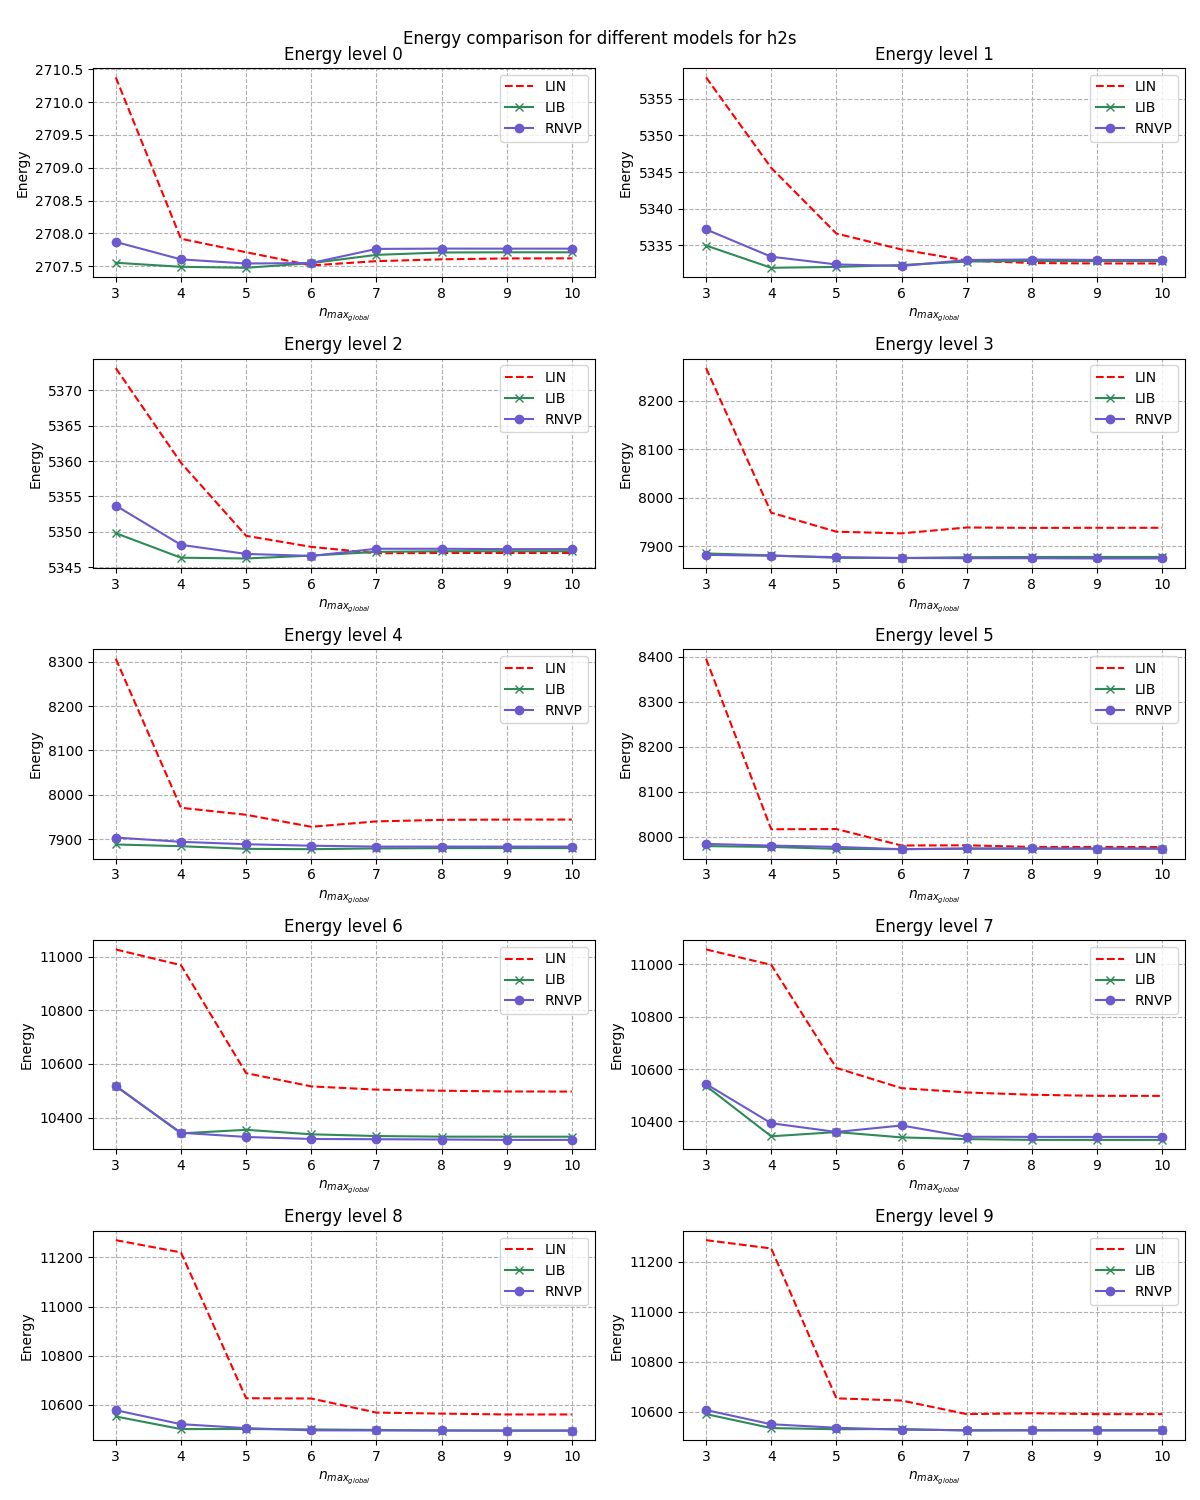
\includegraphics[width=\textheight]{img/enrs_stretch_2D.png}
                \caption{Stretching case for H2S molecule}
                \label{fig:enrs_stretch_2D}
            \end{figure}
        \end{column}
    \end{columns}
\end{frame}
%----------------------------------------------------------------------
% Thank you page is assembled from metadata.tex
\begin{frame}
\frametitle{Thank you!}
\vfill{}
\vspace*{3.5cm}

% check %-% comments for inclusion of a QR code. This is not official
% DESY CD.

\fontsize{8}{9}\selectfont
\begin{columns}
	\hspace*{-0.8em}
	\hspace*{-1em}  % comment if QR code is inserted
	%-% \begin{column}{0.75\textwidth}
	\begin{column}{\textwidth}
		\begin{tabular}{lll}
		\textbf{Contact}&\hspace*{0.5cm} & \\
						&\hspace*{0.5cm} & \\
		\hspace*{-0.4mm}Deutsches Elektronen-&\hspace*{0.5cm} & \AUTHOR\\
		\hspace*{-0.4mm}Synchrotron DESY&\hspace*{0.5cm} & \ORCiD{\ORCID}\\
							&\hspace*{0.5cm} & \GROUP\\
							&\hspace*{0.5cm} & \MailTo{\EMAIL}\\
		\hspace*{-0.4mm}www.desy.de			&\hspace*{0.5cm} & \PHONE\\
							&\hspace*{0.5cm} & \DOIlink{\DOI}\\
		\end{tabular}
	\end{column}
	%-% \begin{column}{0.24\textwidth}
	%-% 
\includegraphics[width=0.8\textwidth]{img/aw-vcf-QRCode}\\
	%-% 	{\tiny\textit{Typeset by lua\LaTeX}}
	%-% \end{column}
\end{columns}


\end{frame}

\end{document}
% Enable spell checker for vim
% setlocal spell spelllang=de


%----------------------------------------------------------------------

% \section{Introduction}
% \subsection{Physics}
% The physical equation governing the setup of the problem is given by the Time Independent Schrödinger's Equation (\textbf{TISE})

% \begin{equation}
%     \HH \ket{\psi} = E \ket{\psi}
%     \label{eq:TISE}
% \end{equation}
% where $\HH$ describes a Hermitian Operator acting on state vectors $\ket{\psi}\in \mathcal{H}$, with real eigenvalues $E$.\\
% For high dimensional systems, this equation can become arbitrarily difficult, with no existing analytical solution for most cases. While several approximations can be made to simplify the scenario itself, the solution can also be approximated numerically without simplifying the scenario.
% \\

% In our case, we will attempt to approximate the groundstate $\ket{\psi_0}$ with a state $\ket{\psi_\Theta}$, and then descend as close as possible to the real state. One way to do this is by minimizing energy eigenvalue as, assuming the eigenstates of $\HH$ form a basis for $\mathcal{H}$, we have that:

% \begin{equation}
%     \boxed{\bra{\psi_{\Theta}} \HH \ket{\psi_\Theta} = \sum_{i, j = 0}^\infty \bar{\alpha}_i\,\alpha_j\bra{\psi_i} \HH\ket{\psi_j} = \sum_{i = 0}^\infty |\alpha_i|^2 E_i \geq \sum_{i = 0}^\infty |\alpha_i|^2 E_0 = E_0}
%     \label{eq:state_E0_ineq}
% \end{equation}
% We can therefore approximate the groundstate energy simply by minimizing the expectation value $\langle \HH \rangle _{\psi_{\Theta}}$.\\
% If we project to a hyperplane orthogonal to the corresponding approximated groundstate $\ket{\widetilde{\psi}_0}$, we have a similar scenario for the next smallest eigenvalue, and can therefore repeat the process to calculate an arbitrary number of eigenstates and eigen-energies.
% \\
% In fact, given a basis for a problem $\{\ket{\varphi_i}\}_i$, we can define the (possibly infinite dimensional) matrices  $\widetilde{H}$ and $S$ with $(\widetilde{H})_{ij} = \bra{\varphi_i}\HH\ket{\varphi_j}$ and $(S)_{ij} = \bra{\varphi_i}\ket{\varphi_j}$, the secular equations \ref{} give the following equation for the eigen-energies:

% \begin{equation}
%     \det\left(\widetilde{H} - E\cdot S\right)
%     \label{eq:secular_eqs}
% \end{equation}

% Which, when $\{\ket{\varphi_i}\}_i$ are orthonormal, have $S$ become the identity matrix and therefore equation \eqref{eq:secular_eqs} becomes analogous to finding the eigenvalues of $\widetilde{H}$.
% % However, the problem has been shifted to the computation of $\langle \HH \rangle _{\psi_{\Theta}}$, as there are infinite terms in this sum. A possible solution is to truncate the degree to which we consider the eigensates. That is, we define a truncation parameter $N_{\max}$ such that we redefine the approximated state as
% However, with an infinite basis these approaches are not in general solvable numerically. A possible solution is to truncate the degree to which we consider the eigensates. That is, we define a truncation parameter $N_{\max}$ such that we redefine the approximated state as

% \begin{equation*}
%     \ket{\psi_{\Theta}} \coloneqq \sum_{k=0}^{N_\text{max}} \alpha_k \ket{\psi_k}
% \end{equation*}

% Then the problem of finding the energies amount to finding eigenvalues of a finite dimensional matrices, which can be approximated numerically. The energies found through the eigenvalues are only approximations to the actual energies, with the errors of these approximations depending on $N_{\max}$. \\It has been shown that, while the energy approximations converge as ${N_{\max} \to \infty}$, this solution suffers from the curse of dimensionality: the parameter $N_{\max}$ depends exponentially on the number of dimensions $d$ of the system for convergence. A possible solution to this problem rises from Machine Learning.

% \subsection{Machine Learning}
% To avoid increasing the parameter $\nmax$ exponentially in relation to $d$, one could consider adding more flexibility to the basis. We will consider coordinate space to achieve this ($\ket{\psi} \equalhat{\psi(x)}$). Given a basis $\{\varphi_i\}_{i}$, we define the augmented basis elements using a coordinate transformation.
% \begin{equation}
%     \varphi^{A}_i(x) = \varphi_i(g(x)) \cdot \sqrt{\det{\frac{\dd g}{\dd x}}}
%     \label{eq:augmented_basis}
% \end{equation}
% where $ \sqrt{\det{\frac{\dd g}{\dd x}}}$ is the square root of the determinant of the Jacobian of this coordinate transformation, which is only used to preserve normalization:
% \begin{align*}
%     \inner{\varphi^A_i}{\varphi^A_j} &= \int \varphi^A_i(x)\cdot{\varphi^A_j(x)}\dd x = \int \varphi_i(g(x))\cdot\varphi_j(g(x))\left({\frac{\dd g}{\dd x}}\right) \dd x  \\
%     &=  \int \varphi_i(g)\cdot\varphi_j(g)\left({\frac{\dd g}{\dd x}}\right) \cdot \frac{\dd x}{\dd g} \dd g = \inner{\varphi_i}{\varphi_j}=1
% \end{align*}

% We can notice that defining a different basis through this form, instead of some, albeit more flexible, arbitrary neural network $\{\text{NN}_i(x)\}_{i=0}^\infty$ ensures two things:
% \begin{itemize}
%     \item The augmented basis elements $\{\varphi^A_i\}_i$ constitute a basis for the space $\mathcal{H}$ when considered without a truncation parameter (which is not given for any set $\{\text{NN}_i\}_i$)
%     \item Orthonormality is preserved between the augmented basis elements $\{\varphi^A_i\}_{i}$
% \end{itemize}
% We also need to impose two further restrictions on the function $g$ for the previous manipulation to be valid: 
% \begin{itemize}
%     \item $g$ must have an inverse
%     \item $g$ must be differentiable and have a differentiable inverse ($g$ must be a diffeomorphism)
% \end{itemize}

% The benefits given using this approach might be subtle: orthonormality preservation is needed to maintain the equivalence between the secular equations and diagonalizing $\widetilde{H}$, while having basis preservation is needed for the convergence of the approximated eigenvalues to the actual eigenvalues as ${\nmax \to \infty}$. \\

% These requirements lead into a possible model for $g$: Normalizing Flows. This model is entirely based on finding diffeomorphisms $\{f_k\}_{k=1}^n$ and composing them (as diffeomorphisms are closed under composition) as follows:
% \begin{equation*}
%     \b{z} = (f_n\circ f_{n-1} \circ \dots \circ f_1 )(\b{x})
% \end{equation*}

% We can then define different schemes for normalizing flows to test the method. 

% \subsection{RNVP model}
% The Real-valued Non-Volume-Preserving model is a type of normalizing flow in which each layer $f_k(x)$ is given by 
% \begin{equation}
%     f_k(x) = \mathcal{P}_k[x] + (\mathbb{1} - \mathcal{P}_k) [g_k(\mathcal{P}_k[x])] \quad \text{with} \quad g_k(z) =  e^{s_k(z)} \odot z + t_k(z)
%     \label{eq:layer_RNVP}
% \end{equation}
%  where $\odot$ denotes the Hadamard or elementwise product, $\mathcal{P}_k$ is a projection over $\lfloor\dim{x}/2\rfloor$ of the components of $x$, and $t_k$ and $s_k$ are arbitrary differentiable functions with same input and output dimension (and with $s_k(x) \neq 0 \;\; \forall x$).  This function is invertible and differentiable with its inverse given by
%  \begin{equation*}
%      f_k^{-1}(z) = \mathcal{P}_k[z] + (\mathbb{1} - \mathcal{P}_k) [g_k^{-1}(\mathcal{P}_k[z])] \quad \text{with} \quad g_k^{-1}(z) =  e^{-s_k(z)} \odot (z - t_k(z))
%  \end{equation*}




